\begin{exercise}
\begin{figure}[H]
\centering
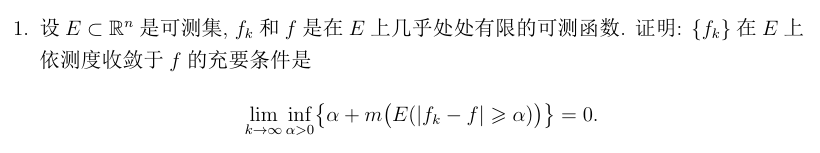
\includegraphics[width=\textwidth]{hw9-2025050523.png}
% \caption{}
\label{}
\end{figure}
\end{exercise}
\begin{proof}
If $f_k\overset{ P }{ \to }f$, then given $\epsilon'>0$, for any $\epsilon>0$, there exists $K=K(\epsilon,\epsilon')>0$, s.t.
\[
m(E(\lvert f_k-f \rvert \geq \epsilon'))<\frac{\epsilon}{2} \qquad \forall k\geq K
\]
Then
\[
\inf_{\alpha>0}\{ \alpha+m(E(\lvert f_k-f \rvert \geq \epsilon')) \}\overset{ \alpha=\frac{\epsilon}{2} }{ \leq } \frac{\epsilon}{2}+m(E(\lvert f_k-f \rvert \geq \epsilon'))<\frac{\epsilon}{2}+\frac{\epsilon}{2}=\epsilon \qquad \forall k\geq K
\]
Thus
\[
\lim_{ k \to \infty } \inf_{\alpha>0}\{ \alpha+m(E(\lvert f_k-f \rvert \geq \alpha)) \}=0
\]
Conversely, suppose that
\[
\lim_{ k \to \infty } \inf_{\alpha>0}\{ \alpha+m(E(\lvert f_k-f \rvert \geq \alpha)) \}=0
\]
i.e. for any $\epsilon>0$, there exists $K=K(\epsilon)>0$, s.t.
\[
\inf_{\alpha>0}\{ \alpha+m(E(\lvert f_k-f \rvert \geq \alpha)) \}<\epsilon \qquad \forall k\geq K
\]
Then there exists $\alpha_0\in(0,\epsilon)$ s.t.
\[
\alpha_0+m(E(\lvert f_k-f \rvert \geq \alpha_0))<\epsilon \qquad \forall k\geq K
\]
Therefore,
\[
m(\underbrace{ E(\lvert f_k-f \rvert \geq \epsilon) }_{ \subset E(\lvert f_k-f \rvert \geq \alpha_0) })\leq m(E(\lvert f_k-f \rvert \geq \alpha_0))<\epsilon-\alpha_0<\epsilon \qquad \forall k\geq K
\]
Given $\epsilon'>0$, for any $\epsilon\in(0,\epsilon')$, we have
\[
m(E(\lvert f_k-f \rvert \geq \epsilon'))\leq m(E(\lvert f_k-f \rvert \geq \epsilon))<\epsilon \qquad \forall k\geq K
\]
Therefore
\[
\lim_{ k \to \infty } m(E(\lvert f_k-f \rvert \geq \epsilon'))=0
\]
\end{proof}

\begin{exercise}
\begin{figure}[H]
\centering
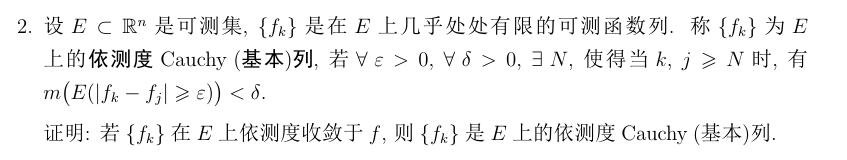
\includegraphics[width=\textwidth]{1-hw9-2025050523.png}
% \caption{}
\label{}
\end{figure}
\end{exercise}
\begin{proof}
Obviously, $f$ is finte a.e. Since $f_k\overset{ P }{ \to }f$, then for given $\epsilon>0$, for any $\delta>0$, there exists $N>0$ s.t.
\[
m\left( E\left( \lvert f_k-f \rvert >\frac{\epsilon}{2} \right) \right)<\frac{\delta}{2}\qquad \forall k\geq N
\]
For any $k,j$, we have
\[
E(\lvert f_k-f_j \rvert \geq \epsilon)\subset E\left( \lvert f_k-f \rvert \geq \frac{\epsilon}{2} \right)\cup E\left( \lvert f_j-f \rvert \geq \frac{\epsilon}{2} \right)
\]
Then for any $k,j\geq N$,
\[
\begin{aligned}
m(E(\lvert f_k-f_j \rvert \geq \epsilon)) & \leq m\left( E\left( \lvert f_k-f \rvert \geq \frac{\epsilon}{2} \right)\cup E\left( \lvert f_j-f \rvert \geq \frac{\epsilon}{2} \right) \right) \\
 & \leq m\left( E\left( \lvert f_k-f \rvert \geq \frac{\epsilon}{2} \right) \right)+m\left( E\left( \lvert f_j-f \rvert \geq \frac{\epsilon}{2} \right) \right) \\
 & <\frac{\delta}{2}+\frac{\delta}{2}=\delta
\end{aligned}
\]
Thus $\{ f_k \}$ is Cauchy in measure.
\end{proof}

\begin{exercise}
\begin{figure}[H]
\centering
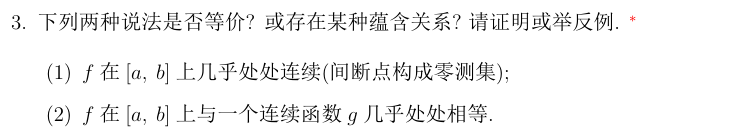
\includegraphics[width=\textwidth]{2-hw9-2025050523.png}
% \caption{}
\label{}
\end{figure}
\end{exercise}
结论:这两种说法既不等价,也不存在蕴含关系。

\begin{proof}

\begin{enumerate}
	\item 证明 $(1) \nRightarrow(2)$
(即:几乎处处连续 不能 推出 几乎处处等于某个连续函数)
	\begin{itemize}
		\item 反例:考虑函数 $f(x)$ 定义在 $[0,1]$ 上:
\[
f(x)= \begin{cases}\sin (1 / x) & \text { if } x \in(0,1] \\ 0 & \text { if } x=0\end{cases}
\]		\item 分析(1):函数 $f(x)$ 在 $(0,1]$ 上是连续的,因为它是由连续函数复合而成的。它仅在 $x=0$ 处不连续,因为当 $x \rightarrow 0^{+}$时, $\sin (1 / x)$ 在 -1 和 1 之间振荡,极限不存在。因此,间断点集合 $D=\{0\}$ 。点集的勒贝格测度为零,所以 $m(D)=0$ 。故函数 $f$ 满足说法(1)。
		\item 分析(2):假设存在一个在 $[0,1]$ 上连续的函数 $g(x)$ ,使得 $f(x)=g(x)$ 几乎处处成立。这意味着集合 $E=\{x \in[0,1] \mid f(x) \neq g(x)\}$ 的测度为零,$m(E)=0$ 。因为 $f(x)$ 和 $g(x)$ 都在 $(0,1]$ 上几乎处处相等,并且它们都在 $(0,1]$ 上连续 ( $g$ 在整个 $[0,1]$ 连续,因此在 $(0,1]$ 连续;$f$ 在 $(0,1]$ 连续),那么它们必须在整个 $(0,1]$ 上都相等。(如果存在 $x_0 \in(0,1]$ 使得 $f\left(x_0\right) \neq g\left(x_0\right)$ ,由连续性,必然存在 $x_0$ 的一个邻域 $\left(x_0-\delta, x_0+\delta\right)$ 使得 $f(x) \neq g(x)$ ,这个区间的测度为 $2 \delta>0$ ,与 $f=g$ 几乎处处矛盾)。因此,必然有 $g(x)=\sin (1 / x)$ 对所有 $x \in(0,1]$ 成立。但是,函数 $\sin (1 / x)$ 在 $x \rightarrow 0^{+}$时极限不存在,所以不可能将它在 $x=0$ 处定义某个值 $g(0)$ 使得 $g(x)$ 在 $x=0$ 处连续。这与 $g(x)$ 是 $[0,1]$ 上的连续函数的前提相矛盾。所以,不存在这样的连续函数 $g(x)$ 。故函数 $f$ 不满足说法(2)。
		\item 结论:(1)不能推出(2)。
	\end{itemize}
	\item 证明 $(2) \nRightarrow(1)$
(即:几乎处处等于某个连续函数 不能 推出 几乎处处连续)
	\begin{itemize}
		\item 反例:考虑狄利克雷函数(Dirichlet function)$f(x)$ 定义在 $[0,1]$ 上:
\[
f(x)= \begin{cases}1 & \text { if } x \in \mathbb{Q} \cap[0,1] \text { (有理数) } \\ 0 & \text { if } x \in[0,1] \backslash \mathbb{Q} \text { (无理数) }\end{cases}
\]		\item 分析(2):令 $g(x)=0$ 对所有 $x \in[0,1]$ 。显然 $g(x)$ 是 $[0,1]$ 上的连续函数。集合 $E=$ $\{x \in[0,1] \mid f(x) \neq g(x)\}=\{x \in[0,1] \mid f(x) \neq 0\}=\mathbb{Q} \cap[0,1]$ 。有理数集合 $\mathbb{Q} \cap[0,1]$ 是可数集,其勒贝格测度为零,即 $m(E)=0$ 。因此,$f(x)$ 与连续函数 $g(x)=0$ 几乎处处相等。故函数 $f$ 满足说法(2)。
		\item 分析(1):狄利克雷函数 $f(x)$ 在 $[0,1]$ 上的每一点都不连续。对于任意 $x_0 \in[0,1]$ ,其任意小的邻域内都既包含有理数( $f$ 值为 1 )也包含无理数( $f$ 值为 0 )。因此 $\lim _{x \rightarrow x_0} f(x)$ 不存在。所以,间断点集合 $D=[0,1]$ 。该集合的勒贝格测度 $m(D)=1 \neq 0$ 。故函数 $f$ 不满足说法 (1)。
		\item 结论:(2)不能推出(1)。
	\end{itemize}
\end{enumerate}

\end{proof}

\begin{exercise}
\begin{figure}[H]
\centering
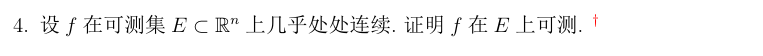
\includegraphics[width=\textwidth]{3-hw9-2025050523.png}
% \caption{}
\label{}
\end{figure}\label{675d91}
\end{exercise}

\begin{proof}
There exists $Z$ with measure 0, s.t. $f$ is continuous thus measurable on $E\setminus Z$. $E\setminus Z$ is clearly measurable. For any open set $\mathcal{O}\subset \mathbb{R}^{n}$,
\[
f^{-1}(\mathcal{O})\setminus(\left.f\right|_{E\setminus Z})^{-1}(\mathcal{O})\subset Z
\]
Since $(\left. f\right|_{E\setminus Z})^{-1}(\mathcal{O})\in \mathcal{M}$ and $m(f^{-1}(\mathcal{O})\setminus(\left.f\right|_{E\setminus Z})^{-1}(\mathcal{O}))=0$, then
\[
f^{-1}(\mathcal{O})\in \mathcal{M}
\]
Thus we are done!

\end{proof}

\begin{exercise}
\begin{figure}[H]
\centering
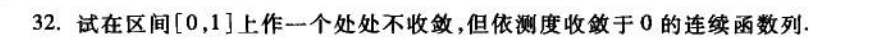
\includegraphics[width=\textwidth]{4-hw9-2025050523.png}
% \caption{}
\label{}
\end{figure}
\end{exercise}
\begin{proof}
Let
\[
f^{(k)}_i(x)=\begin{cases}
1 & x\in\left[ \frac{i-1}{k},\frac{i}{k} \right.\left.\right) \\
0 & \text{elsewhere}
\end{cases}\qquad i=1,2,\dots,k,\quad x\in[0,1]
\]
List these functions
\[
\varphi_1(x)=f_1^{(1)}(x), \quad \varphi_2(x)=f_1^{(2)}(x), \quad \varphi_3(x)=f_2^{(2)}(x), \quad \varphi_4(x)=f_1^{(3)}(x), \quad \cdots
\]
Then $\{ \varphi_n \}\overset{ P }{ \to }0$ on $[0,1]$, because for any $\epsilon\in(0,1)$,
\[
E(\lvert f^{(k)}_{i} \rvert >\epsilon)=\left[ \left.\frac{i-1}{k},\frac{i}{k} \right.\right)
\]
Thus
\[
\lim_{ n \to \infty } m(E(\lvert \varphi _n \rvert >\epsilon ))=\lim_{ k \to \infty } \frac{1}{k}=0
\]
But $\{ \varphi _n \}$ disconverges everywhere on $[0,1]$, since for given $x_0\in[0,1]$, then for any $N>0$, $x_0$ lies in $\left[ \left.\frac{i-1}{k},\frac{i}{k} \right.\right)$ for some $i,k$ large enough ($i+k>2N$), there exists $n_1,n_2>N$, s.t.
\[
\varphi_{n_1}(x_0)=f^{(k)}_i(x_0)=1
\]
\[
\varphi_{n_2}(x_0)=f^{(k)}_{i+1}(x_0)=0
\]
Thus $\varphi _n$ does not converges at $x_0$, by Cauchy's criterion.

We are done!
\end{proof}

\begin{exercise}
\begin{figure}[H]
\centering
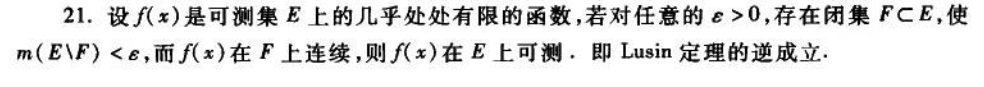
\includegraphics[width=\textwidth]{6-hw9-2025050523.png}
% \caption{}
\label{}
\end{figure}
\end{exercise}
\begin{proof}
For any given $\epsilon>0$, there exists closed $F\subset E$ with $m(E\setminus F)<\epsilon$, s.t. $f$ is continuous on $F$. Then for any open set $\mathcal{O}\subset \mathbb{R}$, we have
\[
(f|_{F})^{-1}(\mathcal{O})\in \mathcal{M}
\]
Note that
\[
(f|_{F})^{-1}(\mathcal{O})=\{ x\in F:f(x)\in \mathcal{O} \}=\{ x\in E:f(x)\in \mathcal{O} \}\cap F=f^{-1}(\mathcal{O})\cap F
\]
For any $A\in \mathcal{M}$, we have
\[
m(A)=m(A\cap(f|_{F})^{-1}(\mathcal{O}))+m(A\cap((f|_{F})^{-1}(\mathcal{O}))^{c})
\]
Note that
\[
\begin{aligned}
A\cap f^{-1}(\mathcal{O}) & =A\cap[(f^{-1}(\mathcal{O})\cap F)\cup(f^{-1}(\mathcal{O})\setminus F)] \\
 & =[A\cap(f|_{F})^{-1}(\mathcal{O})]\cup[A\cap(\underbrace{ f^{-1}(\mathcal{O}) }_{ \subset E }\setminus F)] \\
 & \subset[A\cap(f|_{F}^{-1}(\mathcal{O}))]\cup(E\setminus F)
\end{aligned}
\]
\[
\begin{aligned}
A\cap(f^{-1}(\mathcal{O}))^{c} & =A\cap(E\setminus f^{-1}(\mathcal{O})) \\
 & =A\cap(E\setminus [(f^{-1}(\mathcal{O})\cap F)\cup(f^{-1}(\mathcal{O})\setminus F)]) \\
 & =A\cap(E\cap[(f^{-1}(\mathcal{O})\cap F)\cup(f^{-1}(\mathcal{O})\setminus F)]^{c} ) \\
 & =A\cap E\cap((f|_{F})^{-1}(\mathcal{O}))^{c}\cap(f^{-1}(\mathcal{O})\setminus F)^{c} \\
 & \subset A\cap((f|_{F})^{-1}(\mathcal{O}))^{c}
\end{aligned}
\]
Then
\[
\begin{aligned}
 & \quad m(A\cap f^{-1}(\mathcal{O}))+m(A\cap(f^{-1}(\mathcal{O}))^{c})  \\
 & \leq m(A\cap(f|_{F})^{-1}(\mathcal{O}))+m(A\cap((f|_{F})^{-1}(\mathcal{O}))^{c})+m(E\setminus F) \\
 & \leq m(A)+\epsilon
\end{aligned}
\]
Since $\epsilon$ is arbitrary, we have
\[
m(A\cap f^{-1}(\mathcal{O}))+m(A\cap(f^{-1}(\mathcal{O}))^{c})\leq m(A)
\]
for any open $\mathcal{O}$, thus we are done!

\end{proof}

\begin{exercise}
\begin{figure}[H]
\centering
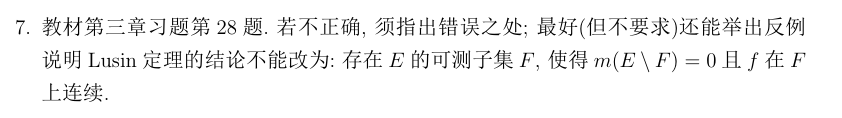
\includegraphics[width=\textwidth]{7-hw9-2025050523.png}
% \caption{}
\label{}
\end{figure}
\begin{figure}[H]
\centering
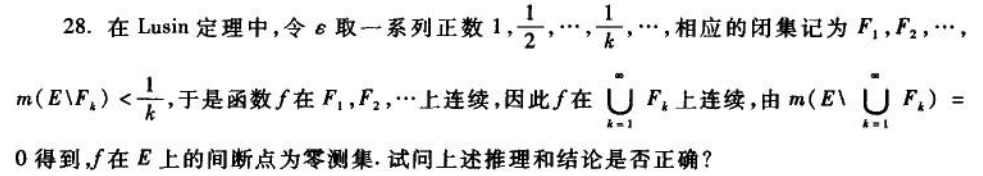
\includegraphics[width=\textwidth]{8-hw9-2025050523.png}
% \caption{}
\label{}
\end{figure}
\end{exercise}
错误在于 $f$ 并不在 $\bigcup_{k=1}^{\infty}F_k$ 上连续,反例考虑
\[
f(x)=\begin{cases}
0 & x\in[0,1] \\
1 & x\in(1,2]
\end{cases}
\]
令 $F_k=\{ 1 \}\cup[1+\frac{1}{k},1]$,显然 $f$ 在 $F_k$ 上连续,但
\[
\bigcup_{k=1}^{\infty } F_k=\{ 1 \}\cup(1,2]=[1,2]
\]
$f(1)=0,f(1,2]=1$,并不连续.

接下来,我们讨论 Lusin 定理的结论是否能改为:存在 $E$ 的可测子集 $F$,使得 $m(E \setminus F)=0$ 且 $f$ 在 $F$ 上连续。并给出反例。

Lusin 定理原文保证存在闭集 $F_\epsilon \subset E$ 使得 $m(E \setminus F_\epsilon) < \epsilon$ 且 $f|_{F_\epsilon}$ 连续。修改后的版本要求:

\begin{enumerate}
	\item $F$ 是可测集 (比闭集更弱的要求)。
	\item $m(E \setminus F)=0$ (比 $m(E \setminus F) < \epsilon$ 更强的要求)。
	\item $f|_F$ 在 $F$ 上连续。
\end{enumerate}

这个修改后的命题不成立。我们可以举出反例。

\begin{example}
令 $E=[0,1]$。构造一个 "Fat Cantor set" (胖康托集) $C \subset [0,1]$。这种集合具有以下性质:
	\begin{enumerate}
		\item $C$ 是闭集 (因此是可测集)。
		\item $C$ 是无处稠密的 (不包含任何区间)。
		\item $C$ 的勒贝格测度 $m(C)>0$。 (例如,在康托三分集的构造中,每次去掉中间 $\frac{1}{3^n}$ 长度的开区间,改为去掉长度为 $\frac{\delta}{3^n}$ 的开区间,其中 $\delta$ 足够小,使得 $\sum \frac{\delta}{3^n} = \frac{\delta}{2} < 1$,则剩余集合的测度为 $1-\frac{\delta}{2}>0$)。
	\end{enumerate}
现在定义函数 $f(x)=\chi_C(x)$,即
\[
f(x)=
\begin{cases}
1 & \text{if } x \in C \\
0 & \text{if } x \in [0,1] \setminus C
\end{cases}
\]由于 $C$ 是可测集,$f(x)$ 是 $E=[0,1]$ 上的可测函数。且 $m(E)=1 < \infty$。
\end{example}
证明 $f(x)$ 不满足修改后的命题:

假设存在一个可测集 $F \subset E=[0,1]$ 使得 $m(E \setminus F)=0$ 且 $f|_F$ 在 $F$ 上连续。

\begin{enumerate}
	\item 由于 $m(E \setminus F)=0$,这意味着 $m(F)=m(E)=1$。
	\item 因为 $m(F)=1$ 且 $m(C)>0$,所以 $F$ 必须与 $C$ 相交,且交集 $F \cap C$ 的测度 $m(F \cap C)=m(C)>0$。(因为 $m(F \cup C)=m(F)+m(C)-m(F \cap C) \leq m(E)=1$,所以 $m(F \cap C) \geq m(F)+m(C)-1=1+m(C)-1=m(C)$。又因为 $F \cap C \subset C, m(F \cap C) \leq m(C)$。故 $m(F \cap C)=m(C)$)。
	\item 同样地,因为 $m(E \setminus F)=0$ 且 $m(E \setminus C)=1-m(C)>0$ (假设 $m(C)<1$),所以 $F$ 必须与 $E \setminus C$ 相交,且 $m(F \cap (E \setminus C))=m(E \setminus C)=1-m(C)>0$。
\end{enumerate}

取一个点 $x \in F \cap C$。因为 $f|_F$ 在 $F$ 上连续,所以 $f|_F$ 在点 $x$ 连续。这意味着:$\lim_{\substack{y \to x \\ y \in F}} f(y)=f(x)$ 由于 $x \in C$,我们有 $f(x)=1$。所以必须有 $\lim_{\substack{y \to x \\ y \in F}} f(y)=1$。

然而,$C$ 是无处稠密的。这意味着在点 $x$ 的任意小邻域 $(x-\delta, x+\delta)$ 内都存在不属于 $C$ 的点。也就是说,存在序列 $y_n \to x$ 使得 $y_n \in E \setminus C$。

由于 $m(E \setminus F)=0$,集合 $E \setminus F$ 不能包含一个测度为 $1-m(C)>0$ 的集合 $E \setminus C$ 的 "大部分"。更确切地说,对于 $x \in C$,由于 $C$ 无处稠密,$x$ 是 $E \setminus C$ 的极限点。因为 $m(F \cap (E \setminus C))=m(E \setminus C)>0$,所以 $F \cap (E \setminus C)$ 不可能是空集,并且它必须在 $x$ 附近积累。因此,我们可以找到一个序列 $y_n \to x$,其中 $y_n \in F \cap (E \setminus C)$。

对于这样的序列 $y_n$:

\begin{enumerate}
	\item $y_n \in F$
	\item $y_n \in E \setminus C$,所以 $f(y_n)=0$。
	\item $y_n \to x$
\end{enumerate}

根据 $f|_F$ 在 $x$ 处连续的要求,我们必须有 $\lim_{n \to \infty} f(y_n)=f(x)$。 但是 $\lim_{n \to \infty} f(y_n)=\lim_{n \to \infty} 0=0$,而 $f(x)=1$。 这导致 $0=1$,产生矛盾。

这个矛盾说明,我们最初的假设(存在满足条件的可测集 $F$)是错误的。

结论: 对于 $f(x)=\chi_C(x)$(其中 $C$ 是胖康托集),不存在可测子集 $F \subset [0,1]$ 使得 $m([0,1] \setminus F)=0$ 且 $f|_F$ 在 $F$ 上连续。这表明 Lusin 定理的结论不能简单地将“闭集 $F_\epsilon$, $m(E \setminus F_\epsilon) < \epsilon$”替换为“可测集 $F$, $m(E \setminus F)=0$”。关键在于 Lusin 定理保证的集合 $F$ 必须是闭集,这提供了更强的拓扑性质,使得限制在其上的函数得以连续。

\begin{exercise}
\begin{figure}[H]
\centering
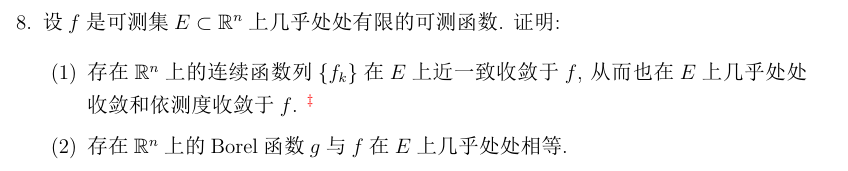
\includegraphics[width=\textwidth]{11-hw9-2025050523.png}
% \caption{}
\label{}
\end{figure}
\end{exercise}
\begin{definition}[近一致收敛]
任给 $\delta>0$,存在 $E$ 的可测子集 $E_\delta$,使在 $E_\delta$ 上 $\left\{f_n\right\}$ 一致收敛于 $f$,而 $m\left(E \backslash E_\delta\right)<\delta$.
\end{definition}
(1)

\begin{note}
只需要 $f_k$ 是可测函数列.
\end{note}
反证而设 $f_k \not\to f$ a.e. 则存在集合 $A\subset E$ , $f_k\not\to f$ 于 $A$,且 $m (A)=\delta>0$. 由于 $\{ f_k \}$ 近一致收敛于 $f$,故存在集合 $E_{\delta}\subset E$,使得
\[
\sup_{x\in E_{\delta}}\lvert f_k(x)-f(x) \rvert \to0
\]
且 $m(E\setminus E_{\delta})<\frac{\delta}{2}$. 断言 $E_{\delta}\cap A\neq \varnothing$,这是因为若 $E_{\delta}\cap A=\varnothing$,那么 $A\subset E\setminus E_{\delta}$,故
\[
\delta=m(A)\leq m(E\setminus E_{\delta})<\frac{\delta}{2}
\]
矛盾. 故存在 $x\in E_{\delta}\cap A$,这意味着
\[
x\in E_{\delta}\Rightarrow\lvert f_k(x)-f(x) \rvert \to0
\]
\[
x\in A\Rightarrow \lvert f_k(x)-f(x) \rvert \not\to0
\]
矛盾!故近一致收敛蕴含几乎处处收敛.

\begin{remark}
注意:当 $mE=\infty$ 时,几乎处处收敛并不蕴含依测度收敛.
\end{remark}
反证而设 $f_k\overset{ P }{ \to }f$, 则存在 $\epsilon_0>0$,使得 $m (E (\lvert f_k-f \rvert>\epsilon_0))\not\to0$,也就是存在 $\delta>0,N>0$,使得
\[
m(\underbrace{ E(\lvert f_k-f \rvert >\epsilon_0) }_{ \eqqcolon \widetilde{E} })\geq \delta \qquad \forall k\geq N
\]
由于 $\{ f_k \}$ 近一致收敛于 $f$,故存在集合 $E_{\delta}\subset E$,使得
\[
\sup_{x\in E_{\delta}}\lvert f_k(x)-f(x) \rvert \to0
\]
且 $m(E\setminus E_{\delta})<\frac{\delta}{2}$. 也就是存在 $N'>0$,使得
\[
\sup_{x\in E_{\delta}}\lvert f_k(x)-f(x) \rvert <\epsilon_0 \qquad \forall k\geq N'
\]
我们任取 $k\geq \max\{ N,N' \}$,固定 $k$ ,由于 $m(\widetilde{E})\geq\delta$, $m(E\setminus E_{\delta})<\frac{\delta}{2}$,那么 $\widetilde{E}\cap E_{\delta}\neq \varnothing$, 于是存在 $x\in \widetilde{E}\cap E_{\delta}$,故
\[
x\in \widetilde{E}\Rightarrow \lvert f_k(x)-f(x) \rvert >\epsilon_0
\]
\[
x\in E_{\delta}\Rightarrow \lvert f_k(x)-f(x) \rvert <\epsilon_0
\]
矛盾!故近一致收敛蕴含依测度收敛.

\begin{exercise}
\begin{figure}[H]
\centering
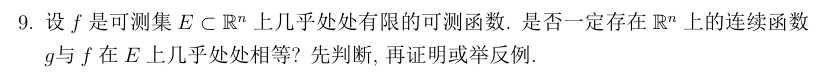
\includegraphics[width=\textwidth]{9-hw9-2025050523.png}
% \caption{}
\label{}
\end{figure}
\end{exercise}
判断:不一定存在这样的连续函数 $g$。

\begin{proof}
(举反例) 考虑 $n=1$ 的情况。令可测集 $E = [0,1] \subset \mathbb{R}$。

令 $C \subset (0,1)$为一个“胖”康托集(generalized Cantor set)。这样的集合 $C$ 具有以下性质:

\begin{enumerate}
	\item $C$ 是闭集。
	\item $C$ 是无处稠密集(nowhere dense),即 $C$ 的闭包(就是 $C$ 本身)不包含任何开区间。因此其内部为空。
	\item $C$ 的勒贝格测度 $m(C) > 0$。
\end{enumerate}

定义 $E$ 上的可测函数 $f: E \to \mathbb{R}$ 为 $f(x) = \chi_C(x)$,即 $C$ 的特征函数。
\[
f(x) = \begin{cases} 1, & x \in C \\ 0, & x \in [0,1] \setminus C \end{cases}
\]
这个函数 $f$ 在 $E$ 上显然是可测的(因为 $C$ 是闭集,故为可测集),并且几乎处处有限(实际上处处有限,其值仅为0或1)。

现在,我们假设存在一个在 $\mathbb{R}$ 上连续的函数 $g: \mathbb{R} \to \mathbb{R}$,使得 $f$ 与 $g$ 在 $E$ 上几乎处处相等。这意味着集合 $\{x \in E \mid f(x) \neq g(x)\}$ 的勒贝格测度为0。
即 $m(\{x \in [0,1] \mid f(x) \neq g(x)\}) = 0$。

令 $U = (0,1) \setminus C$。由于 $C$ 是闭集且 $C \subset (0,1)$,所以 $U$ 是 $\mathbb{R}$ 中的一个开集(它是一些互不相交的开区间的并集)。
对于 $x \in U$,我们有 $f(x) = 0$。
由于 $f=g$ 在 $E$ 上几乎处处相等,所以 $g(x) = 0$ 对于几乎所有 $x \in U$ 成立。
设 $N_0 = \{x \in U \mid g(x) \neq 0\}$。则 $N_0 \subset \{x \in E \mid f(x) \neq g(x)\}$,所以 $m(N_0)=0$。
因此,$g(x)=0$ 在 $U \setminus N_0$ 上成立,其中 $m(U \setminus N_0) = m(U)$。
由于 $g$ 是连续函数,且 $U$ 是开集,若 $g$ 在 $U$ 的一个具有全测度的子集上为0,则 $g$ 必须在整个 $U$ 上为0。
(详细说明:假设存在一点 $x_0 \in U$ 使得 $g(x_0) \neq 0$。由于 $g$ 连续,存在一个以 $x_0$ 为中心的小开区间 $I \subset U$ 使得 $g(x) \neq 0$ 对所有 $x \in I$ 成立。但这意味着 $m(\{x \in U \mid g(x) \neq 0\}) \ge m(I) > 0$,这与 $g(x)=0$ 对几乎所有 $x \in U$ 矛盾。因此,$g(x)=0$ 对所有 $x \in U$ 成立。)

因为 $C$ 是 $(0,1)$ 中的无处稠密集,所以 $U = (0,1) \setminus C$ 在 $(0,1)$ 中是稠密的。这意味着 $\text{cl}(U)$ ( $U$ 在 $\mathbb{R}$ 中的闭包) 包含 $(0,1)$。更准确地说,$\text{cl}(U) = \text{cl}((0,1) \setminus C) = [0,1]$ (因为 $C$ 不包含任何区间,且 $C \subset (0,1)$)。
对于任何一点 $y \in C$,由于 $C$ 是无处稠密集,$y$ 是 $U$ 的一个聚点。因此,存在一个序列 $(x_k)$,其中 $x_k \in U$,使得 $x_k \to y$。
由于 $g$ 是连续函数,且 $g(x_k)=0$ 对于所有 $x_k \in U$,我们有:
\[
g(y) = \lim_{k \to \infty} g(x_k) = \lim_{k \to \infty} 0 = 0
\]
这表明 $g(y)=0$ 对于所有 $y \in C$ 成立。

结合 $g(x)=0$ 对所有 $x \in U$ 和 $g(y)=0$ 对所有 $y \in C$,我们得到 $g(x)=0$ 对所有 $x \in U \cup C = (0,1)$ 成立。
由于 $g$ 在 $\mathbb{R}$ 上是连续的,所以 $g(x)=0$ 对所有 $x \in \text{cl}((0,1)) = [0,1]$ 成立。
也就是说,$g(x)=0$ 对所有 $x \in E = [0,1]$ 成立。

现在我们比较 $f$ 和 $g$ 在 $E$ 上的差异:
$f(x) = \chi_C(x)$
$g(x) = 0$ 对于所有 $x \in [0,1]$。
那么,$f(x) \neq g(x)$ 当且仅当 $\chi_C(x) \neq 0$,这意味着当且仅当 $x \in C$。
所以,集合 $\{x \in E \mid f(x) \neq g(x)\} = C$。
为了使得 $f$ 和 $g$ 在 $E$ 上几乎处处相等,这个集合的测度必须为0,即 $m(C)=0$。
但这与我们选择 $C$ 为一个具有正测度($m(C)>0$)的胖康托集相矛盾。

因此,我们的初始假设(即存在这样的连续函数 $g$)是错误的。
所以,不一定存在 $\mathbb{R}^n$ 上的连续函数 $g$ 与 $f$ 在 $E$ 上几乎处处相等。

这个反例可以推广到 $\mathbb{R}^n$ ($n>1$)。例如,取 $E = [0,1]^n$。令 $C_0 \subset (0,1)$ 为如上定义的胖康托集。令 $A = C_0 \times [0,1]^{n-1} \subset E$。则 $A$ 是 $E$ 中的闭集、无处稠密集,且其 $n$ 维勒贝格测度 $m_n(A) = m_1(C_0) \cdot (m_1([0,1]))^{n-1} = m_1(C_0) > 0$。定义 $f(x) = \chi_A(x)$。通过与上述类似的论证,可以证明不存在满足题设条件的连续函数 $g:\mathbb{R}^n \to \mathbb{R}$。核心步骤是证明若 $g$ 存在,则 $g$ 必须在 $(0,1)^n$ 上为0,进而利用 $g$ 的连续性推广到 $g$ 在 $E=[0,1]^n$ 上为0,从而导致 $m_n(\{x \in E \mid f(x) \neq g(x)\}) = m_n(A) > 0$,产生矛盾。
\end{proof}

\begin{exercise}
\begin{figure}[H]
\centering
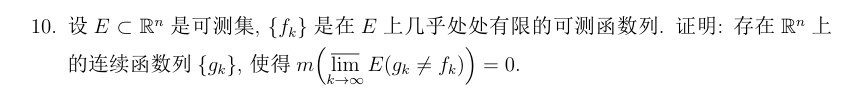
\includegraphics[width=\textwidth]{10-hw9-2025050523.png}
% \caption{}
\label{}
\end{figure}
\end{exercise}
\begin{proof}
由于 $f_k$ 可测,则由 Lusin 引理,存在闭集 $F_k\subset E$ 和 $\mathbb{R}^{n}$ 上的连续函数 $g_k$,使得
\[
f_k=g_k\text{ on }F_k\text{ and }m(E\setminus F_k)<\frac{1}{2^{k}}
\]
于是
\[
E(g_k\neq f_k)\subset E\setminus F_k\implies m(E(g_k\neq f_k))\leq m(E\setminus F_k)<\frac{1}{2^{k}}
\]
这样构造出一列 $\{ g_k \}$,从而
\[
\begin{aligned}
m(\varlimsup_{ k \to \infty } E(g_k\neq f_k)) & =m\left( \bigcap_{k=1}^{\infty} \bigcup_{n=k}^{\infty} E(g_n\neq f_n) \right) \\
 & \leq m\left( \bigcup_{n=k}^{\infty} E(g_n\neq f_n) \right) \\
 & \leq \sum_{n=k}^{\infty} m(E(g_n\neq f_n)) \\
 & \leq \sum_{n=k}^{\infty} \frac{1}{2^{n}} \\
 & =\frac{1}{2^{k-1}}\qquad \forall k
\end{aligned}
\]
由 $k$ 的任意性可知
\[
m(\varlimsup_{ k \to \infty } E(g_k\neq f_k))=0
\]
\end{proof}
